\subsection{Présentation du CNRS}
Le CNRS, ou Centre National de la Recherche Scientifique, est une institution de recherche parmi les plus importantes au monde. Pour relever les grands défis présents et à venir, ses scientifiques explorent le vivant, la matière, l’Univers et le fonctionnement des sociétés humaines. Mondialement reconnu pour l’excellence de ses travaux scientifiques, le CNRS est une référence, aussi bien dans l’univers de la recherche et du développement, que pour le grand public. Le CNRS étant une importante entreprise publique, les domaines de recherches sont très vastes (sciences, langues, histoires, mathématiques \ldots). 

\subsection{Présentation de l'IFSeM}
\textit{"Créé en juillet 2015, le Service Mutualisé d’Île-de-France, rattaché à la Délégation Paris-Villejuif, prend en charge des activités jusqu’alors exercées par les 5 délégations franciliennes et les regroupe en 4 pôles de compétences au bénéfice de toutes\footnotemark. "}
\footnotetext{https://www.dr1.cnrs.fr/spip.php?rubrique59}
\smallbreak
Voici ce que l'on peut lire sur le site de la délégation Ile-de-France-Villejuif du CNRS. Comme expliqué en introduction, l'IFSeM est situé à Villejuif, sur le même campus que la délégation régionale numéro 1 (DR01). L'IFSeM est constitué de 4 pôles : Formation, Achats, Système d'information et Patrimoine immobilier. Ces pôles ont pour mission de "gagner en cohérence et permettre à toutes les délégations d'Ile-de-France d’apporter le meilleur niveau de service à ses unités comme à son personnel".

\subsection{Présentation du pôle SI de l'IFSEM}
J'ai donc choisi, dans la continuité de mon projet à ESIEE Paris, d'effectuer ce stage d'un mois au pôle informatique de l'IFSeM, dans l'équipe infrastructure. 
Ce pôle a pour objectif d'apporter une assistance technique à 4 délégations différentes du CNRS : la DR01, située à Villejuif, la DR02, à Paris-Centre, la DR04 à Gif-Sur-Yvettes et la DR05 située à Meudon. De plus, ce service a pour but de maintenir et mettre à jour les applications nationales du CNRS au travers de différents serveurs décentralisés. 
\newpage
\subsection{Fonctionnement de l'entreprise : Le travail en équipe}

Le pôle informatique de l'IFSeM est divisé en 3 équipes (pour l'organigramme complet, se reporter, en annexe, au point 5.1.1) : 
\begin{itemize}
    \item Le support aux applications et offre de services : \textit{"support et exploitation de la téléphonie IP après déploiement, support des applications nationales du CNRS, création et accompagnement de la mise en oeuvre de l’offre de services nationale pour les délégations concernées et les laboratoires qui en dépendent.\footnotemark[3]"}
    \item La gestion des infrastructures : \textit{"gestion de parc informatique, sécurité informatique (communication/formation à destination des unités, support à la gestion des incidents), et gestion des systèmes et réseaux (support à l’ingénierie, gestion propre au Service Mutualisé, supervision des raccordements de sites).\footnotemark[3]"}
    \item Le développement logiciel : \textit{"besoins applicatifs propres au Service Mutualisé et applications métiers recouvrant les besoins communs aux 5 délégations.\footnotemark[3]"}
\end{itemize}
\footnotetext[3]{Voir note 2}
\smallbreak
Durant mon stage, j'ai été affecté à l'équipe "Gestion des infrastructures". J'étais dans un bureau de 4 personnes. J'ai pu observer que les trois équipes collaboraient au travers d'échanges et de discussions, et chacun apportait son aide et participait à la recherche de solutions des autres groupes. 
Ces trois équipes sont sous la direction de Mr Etienne FAURE, Ingénieur de Recherches.

\subsubsection{Le ticketing}
Une machine virtuelle faisant tourner un serveur OTRS (Open-source Ticket Request System) permet aux utilisateurs qui rencontrent un problème de le notifier au travers d'un ticket d'assistance aux 3 équipes du SI. \\
Le ticketing est la méthodologie qui est employée pour la résolutions des faits techniques remontés par les utilisateurs :
\begin{itemize}
    \item L'utilisateur ouvre un ticket depuis un site internet
    \item En fonction du type de problème, l'équipe concerné (support, infra ou dev) prend en charge le ticket.
    \item Si le problème concerne un seul utilisateur, une fois résolu, le ticket est fermé.
    \item Si le problème concerne plusieurs utilisateurs, on applique des GPO (Group Policy Object). C'est un ensemble de règles qui sont appliquées de différentes façons (à tous les ordinateurs, tous les utilisateurs, un groupe, une seule personne, un service ...). C'est ce que l'on appelle une stratégie de groupe. Cela permet de corriger le problème pour tout le monde, et non au cas par cas.
\end{itemize}
Dès l'instant où le ticket est pris en charge, il disparaît de l'écran des autres membres du SI, afin de faciliter son traitement et d'éviter les doublons, ce qui ferait perdre beaucoup de temps. Cela n'empêche en rien les autres équipes d'apporter leur aide à la personne qui a bloqué le ticket. En effet, toutes les personnes ayant lu le message sont au courant du problème et peuvent apporter leur aide.\\
\vspace{2\baselineskip}
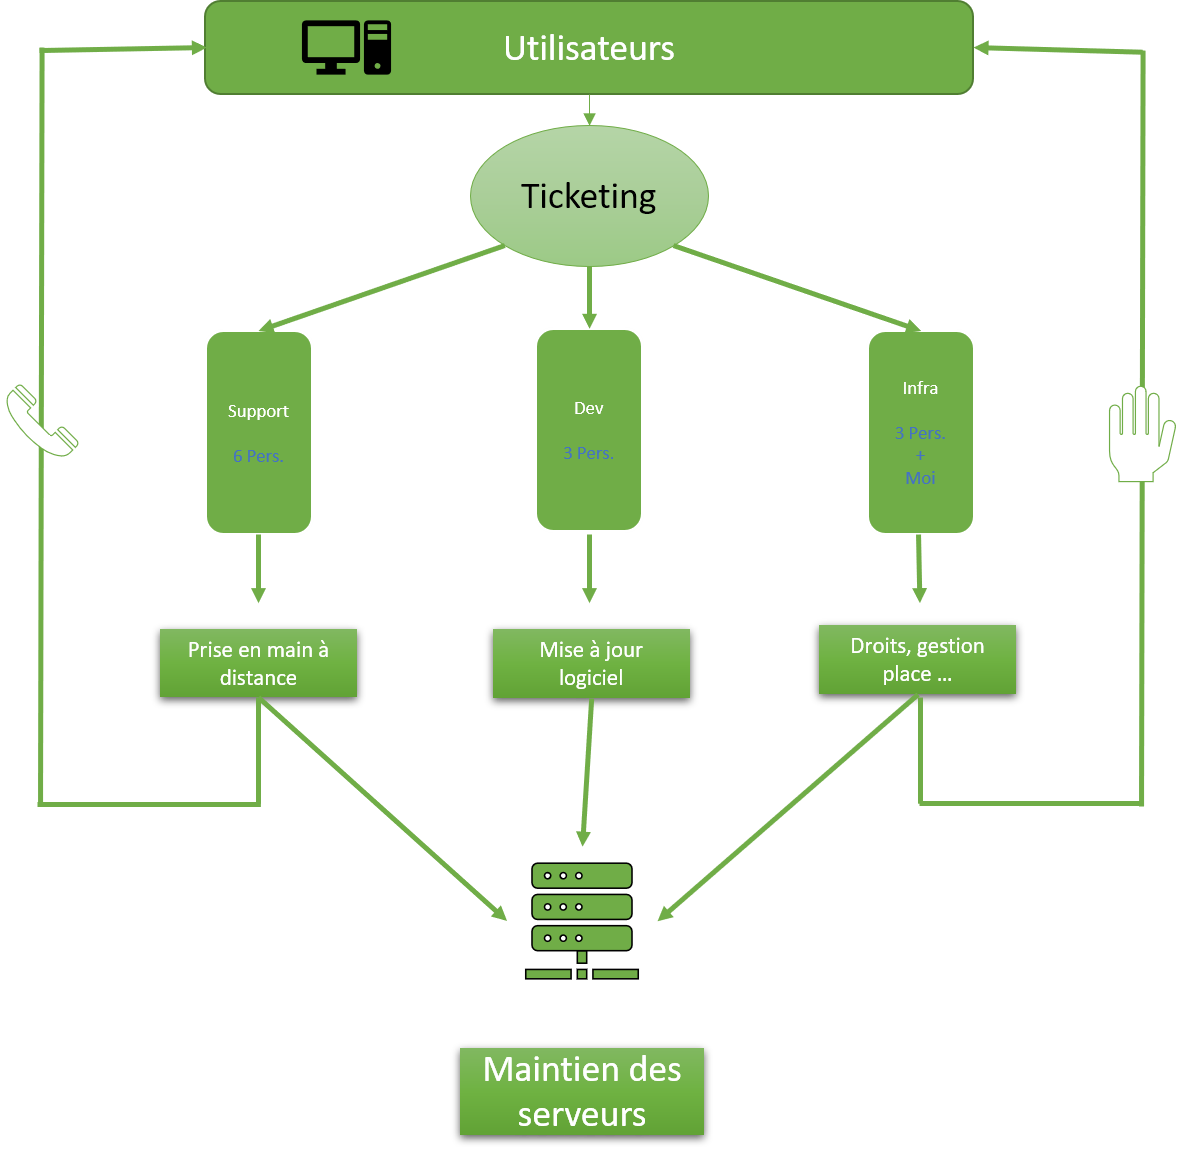
\includegraphics[width=15cm]{./images/orga.png}
\newpage

\subsubsection{Coordination intra-équipe}
La coordination intra-équipe est facile et naturelle. En effet, les bureaux sont composés d'un petit nombre de personne, mais toujours 2 au minimum. De plus, les équipes sont assez restreintes, entre 3 et 6 personnes au maximum pour l'équipe support. La communication se fait donc naturellement. Lorsqu'un membre d'une équipe a un problème, une demande ou une information à faire passer, il peut simplement en parler avec les autres membres de son équipes. 
De plus, les bureaux étant occupés par des membres d'une même équipe, cela facilite les échanges, et on peut parler assez fort sans risquer de gêner les autres équipes qui sont dans des bureaux différents. 

\subsubsection{Coordination inter-équipe}
De par la séparation des bureaux évoquée au paragraphe précédent, il à été mis en place des réunions de service, regroupant une partie ou l'entièreté du pôle SI, afin de d'échanger sur des sujets communs. \\
Un exemple de réunion à laquelle j'ai assisté est la réunion mensuelle organisée par Baptiste BARAKOWSKY, responsable de l'équipe "Gestion des infrastructures", afin d'expliciter les différents GPO qui sont appliquées par l'IFSeM. En effet, plus le nombre de problème augmente, plus le nombre de GPO est important. Cette réunion à donc pour but d'informer les autres équipes des correctifs qui sont déjà appliqués.

\subsubsection{Des échanges informels au service du groupe}
La communication et la cohésion de groupe étant primordiale dans ce genre d'organisation, la "pause café" se révèle constructive au sein d'un groupe comme celui-là. En effet, selon les statistiques, 84\% des salariés jugent important d'avoir une machine à café à disposition dans les locaux de l'entreprise. Cela permet de développer la solidarité entre les membres des différentes équipes, en plus d'être un lieu de détente et d'échanges.
\smallbreak
Dans le cas de l'IFSeM, ces pauses permettait un échange entre les différentes équipes, et même avec les différents pôles de l'IFSeM. Cela permet aux personnels d'échanger, aussi bien sur le plan professionnel que personnel. 
Ces pauses permettent une bonne ambiance de travail et une certaine complicité entre les membres des différentes équipes, qui ne peut qu'être bénéfique au service. En effet, si les personnes s'entendent bien entre elles, le dialogue en est facilité.  

\subsubsection{Moyens de communications internes}
Le CNRS, comme de nombreuses organisations de cette taille, dispose de différents moyens de communications qui sont plus ou moins utilisés :
\begin{itemize}
    \item Le téléphone : chaque agent dispose d'un téléphone IP dans son bureau. Dans le cas du SI, ce téléphone sert uniquement à communiquer avec les utilisateurs qui ont besoin d'aide;
    \item Les mails : l'envoi de mails est soit officiel (administratifs, échanges avec l'extérieur du CNRS\dots) soit interne. Dans ce cas, les mails servent principalement pour garder une trace écrite sans encombrer le disque dur, soit pour transférer des documents (Word par exemple).
    \item La messagerie instantanée : l'utilisation de messagerie instantanées permet aux employés de créer des groupes, de discuter, d'envoyer des informations, de poser des questions\dots depuis leurs bureaux respectifs. Cela permet premièrement de gagner du temps, par rapport aux mails par exemple, mais aussi d'être plus multi-tâche. En effet, on peut très bien parler au téléphone avec un utilisateur et poser une question à un autre membre de l'équipe, sans pour autant être gêné dans son travail.
\end{itemize}